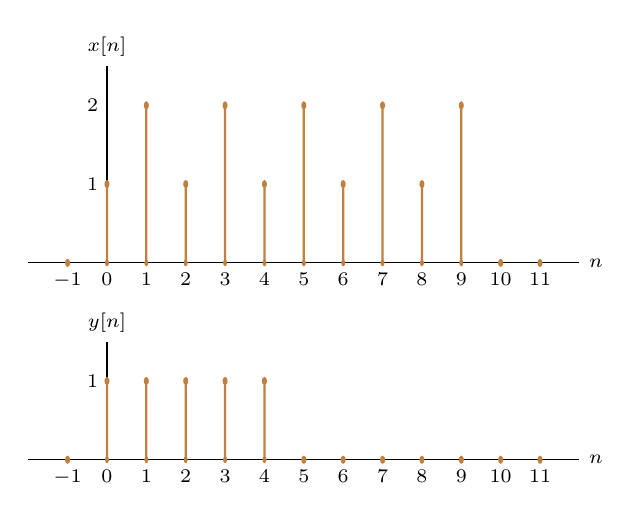
\begin{tikzpicture}[xscale=0.5]




	\def\nmin{-1}
	\def\nmax{11}	
	
	\begin{scope}	
		\def\x{{0, 1, 2, 1, 2, 1, 2, 1, 2, 1, 2, 0, 0}}	

		\draw (\nmin-1, 0) -- (\nmax+1, 0) node[anchor=west] {\scriptsize $n$};
		\draw (0,0) -- ++(0, 2.5) node [anchor=south] {\scriptsize $x[n]$};
% 		\foreach \n/\l in {-1/{-N_1}, 1/0, 3/{N_1}}
% 		{
% 			\node at (\n/4, 0) [anchor=north] {\scriptsize $\l$};
% 		}
		\foreach \n in {-1, 0, ..., 11}
		{
			\node at (\n, 0) [anchor=north] {\scriptsize $\n$};
		}
		\node at (-0.75,1) [anchor=west] {\scriptsize $1$};
		\node at (-0.75,2) [anchor=west] {\scriptsize $2$};
		
		\foreach \n in {0,1, ..., 12}
		{
			\pgfmathparse{\x[\n]}
			\edef\xn{\pgfmathresult}	
			\ifthenelse{\xn > 0}
			{
				\draw[brown, thick, fill=brown]  (\n + \nmin, 0) -- ++(0, \xn) circle (1pt);% node[anchor=east] {\scriptsize $\xn$};
			}
			{
				\draw[brown, fill=brown] (\n+ \nmin,  0) circle (1pt);
			}
		}
	\end{scope}		
	
	\begin{scope}[yshift=-2.5cm]	
		\def\x{{0, 1, 1, 1, 1, 1, 0, 0, 0, 0, 0, 0, 0}}	

		\draw (\nmin-1, 0) -- (\nmax+1, 0) node[anchor=west] {\scriptsize $n$};
		\draw (0,0) -- ++(0, 1.5) node [anchor=south] {\scriptsize $y[n]$};
% 		\foreach \n/\l in {-1/{-N_1}, 1/0, 3/{N_1}}
% 		{
% 			\node at (\n/4, 0) [anchor=north] {\scriptsize $\l$};
% 		}
		\foreach \n in {-1, 0, ..., 11}
		{
			\node at (\n, 0) [anchor=north] {\scriptsize $\n$};
		}
		\node at (-0.75,1) [anchor=west] {\scriptsize $1$};

		
		\foreach \n in {0,1, ..., 12}
		{
			\pgfmathparse{\x[\n]}
			\edef\xn{\pgfmathresult}	
			\ifthenelse{\xn > 0}
			{
				\draw[brown, thick, fill=brown]  (\n + \nmin, 0) -- ++(0, \xn) circle (1pt);% node[anchor=east] {\scriptsize $\xn$};
			}
			{
				\draw[brown, fill=brown] (\n+ \nmin,  0) circle (1pt);
			}
		}
	\end{scope}	
\end{tikzpicture}